\providecommand{\main}{../../../..}
\documentclass[\main/dresen_thesis.tex]{subfiles}
  \renewcommand{\thisPath}{\main/chapters/monolayers/structureModel/squareArrayParacrystal}

\begin{document}
  \label{sec:monolayers:structure:squareArrayParacrystalGISAXS}
  \begin{figure}[tb]
    \centering
    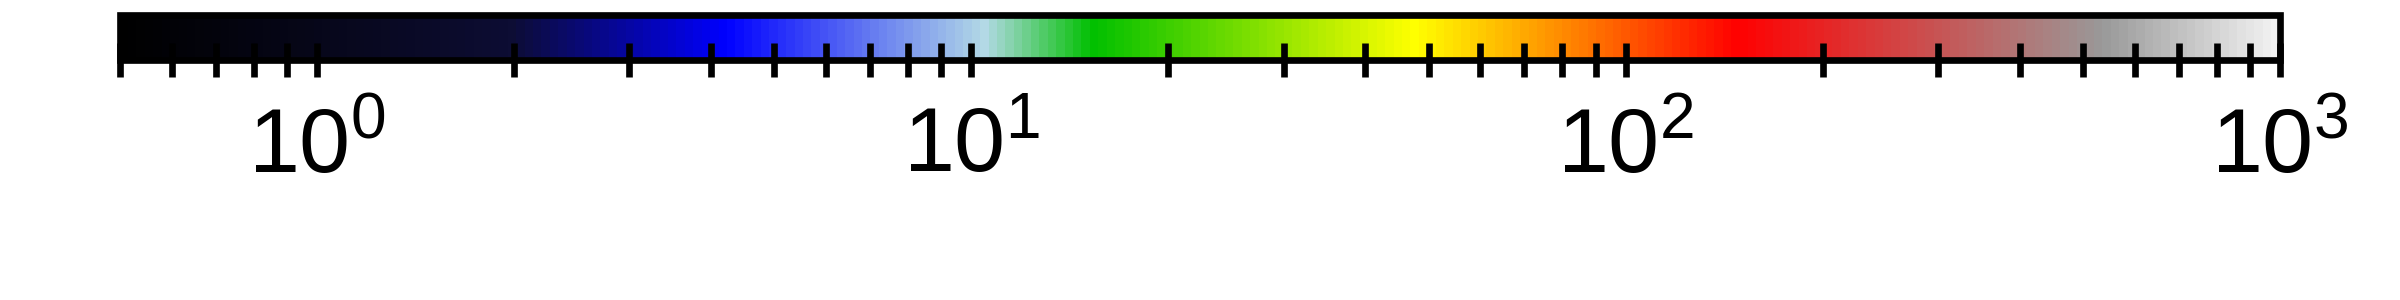
\includegraphics{monolayers_ML-Ac-CoFe-C_GISAXS_SVcbar}
    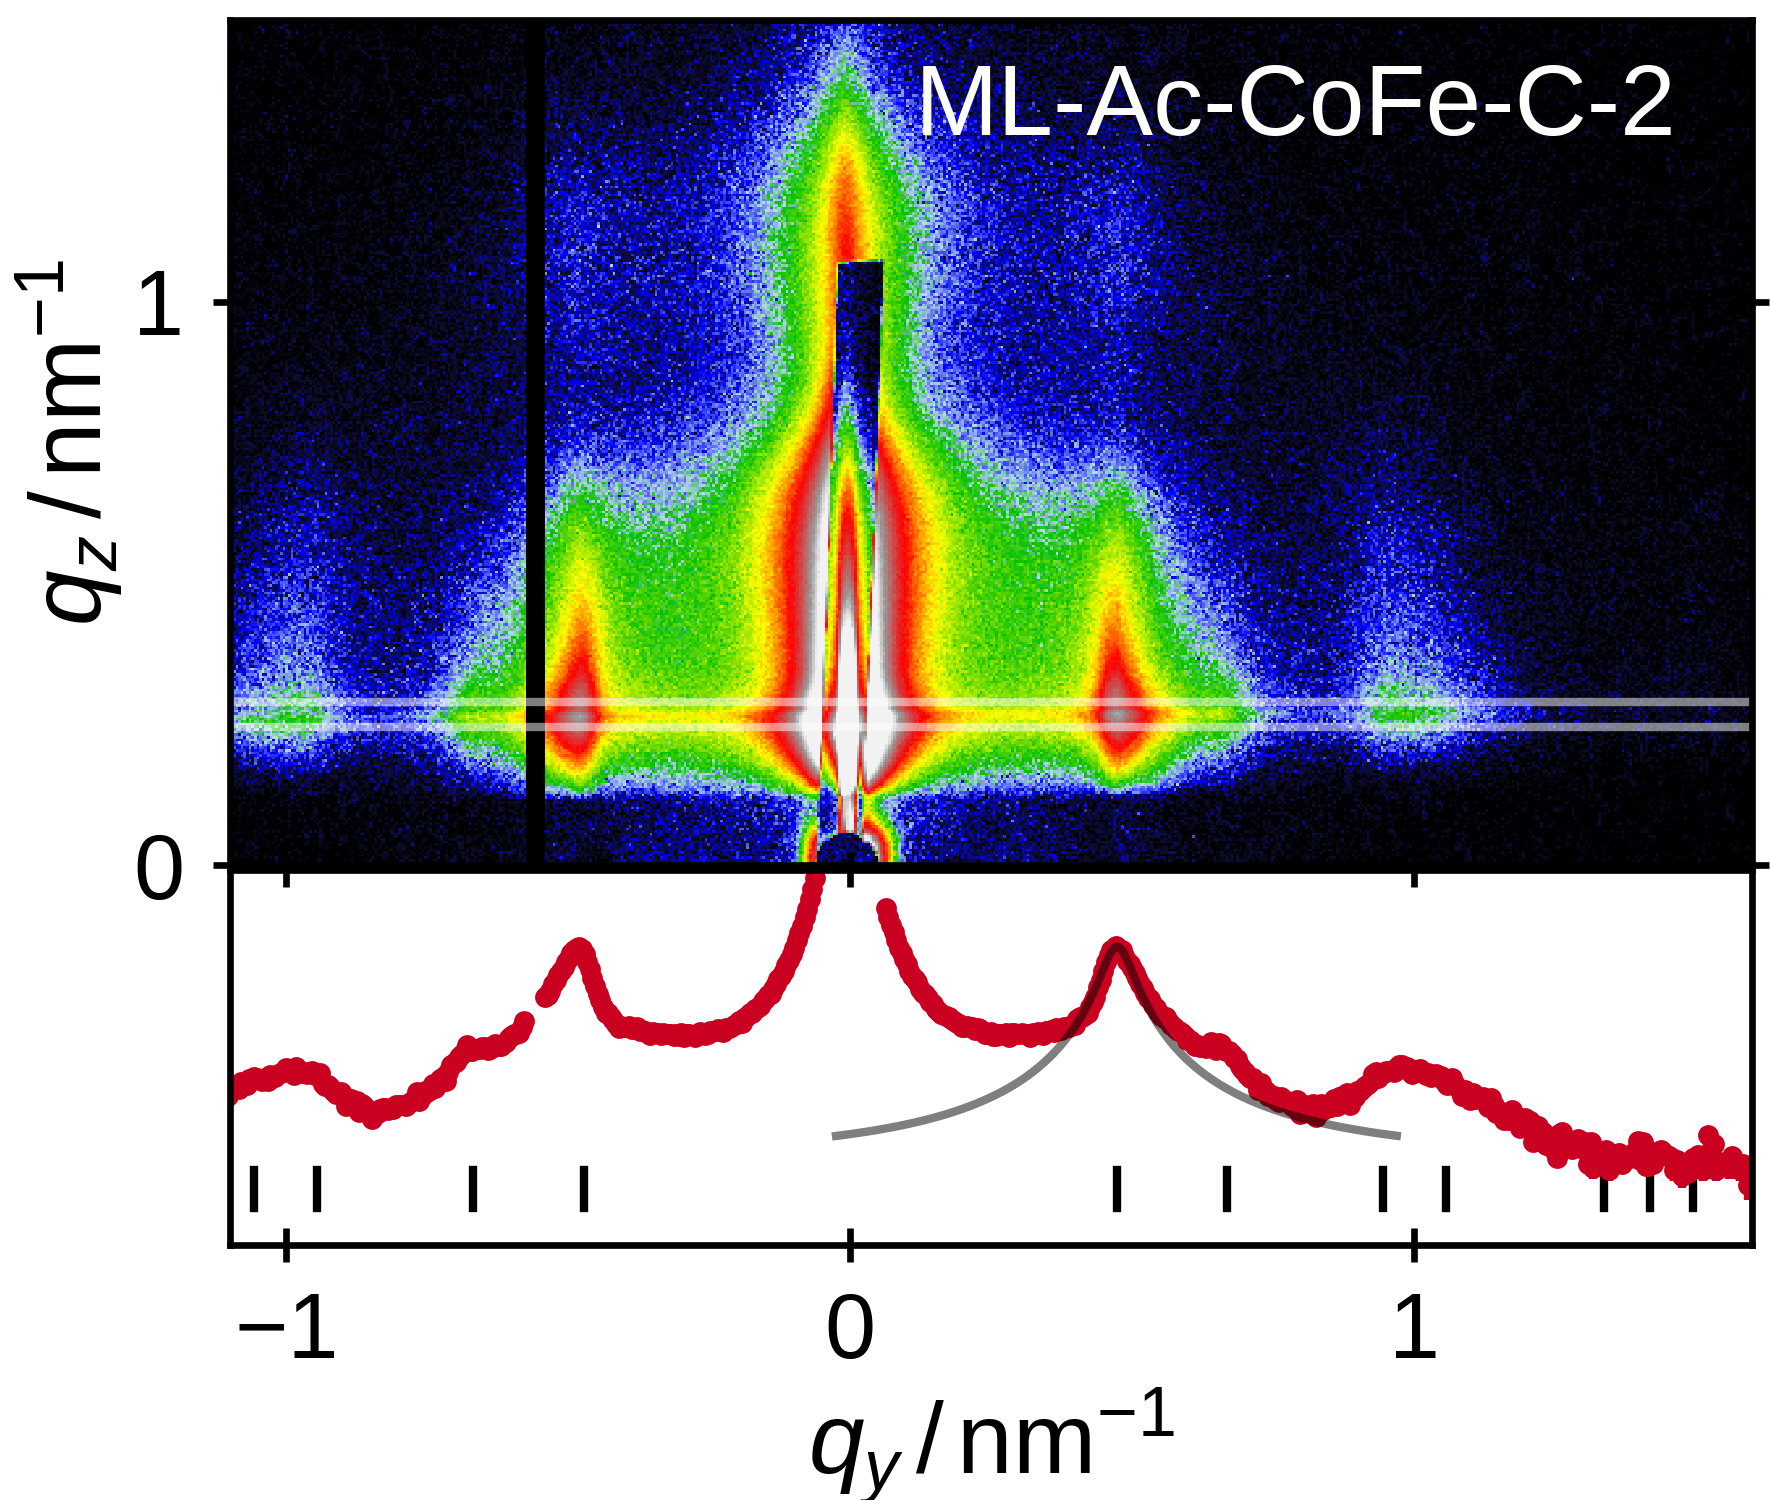
\includegraphics{monolayers_GISAXS_ML-Ac-CoFe-C-2}
    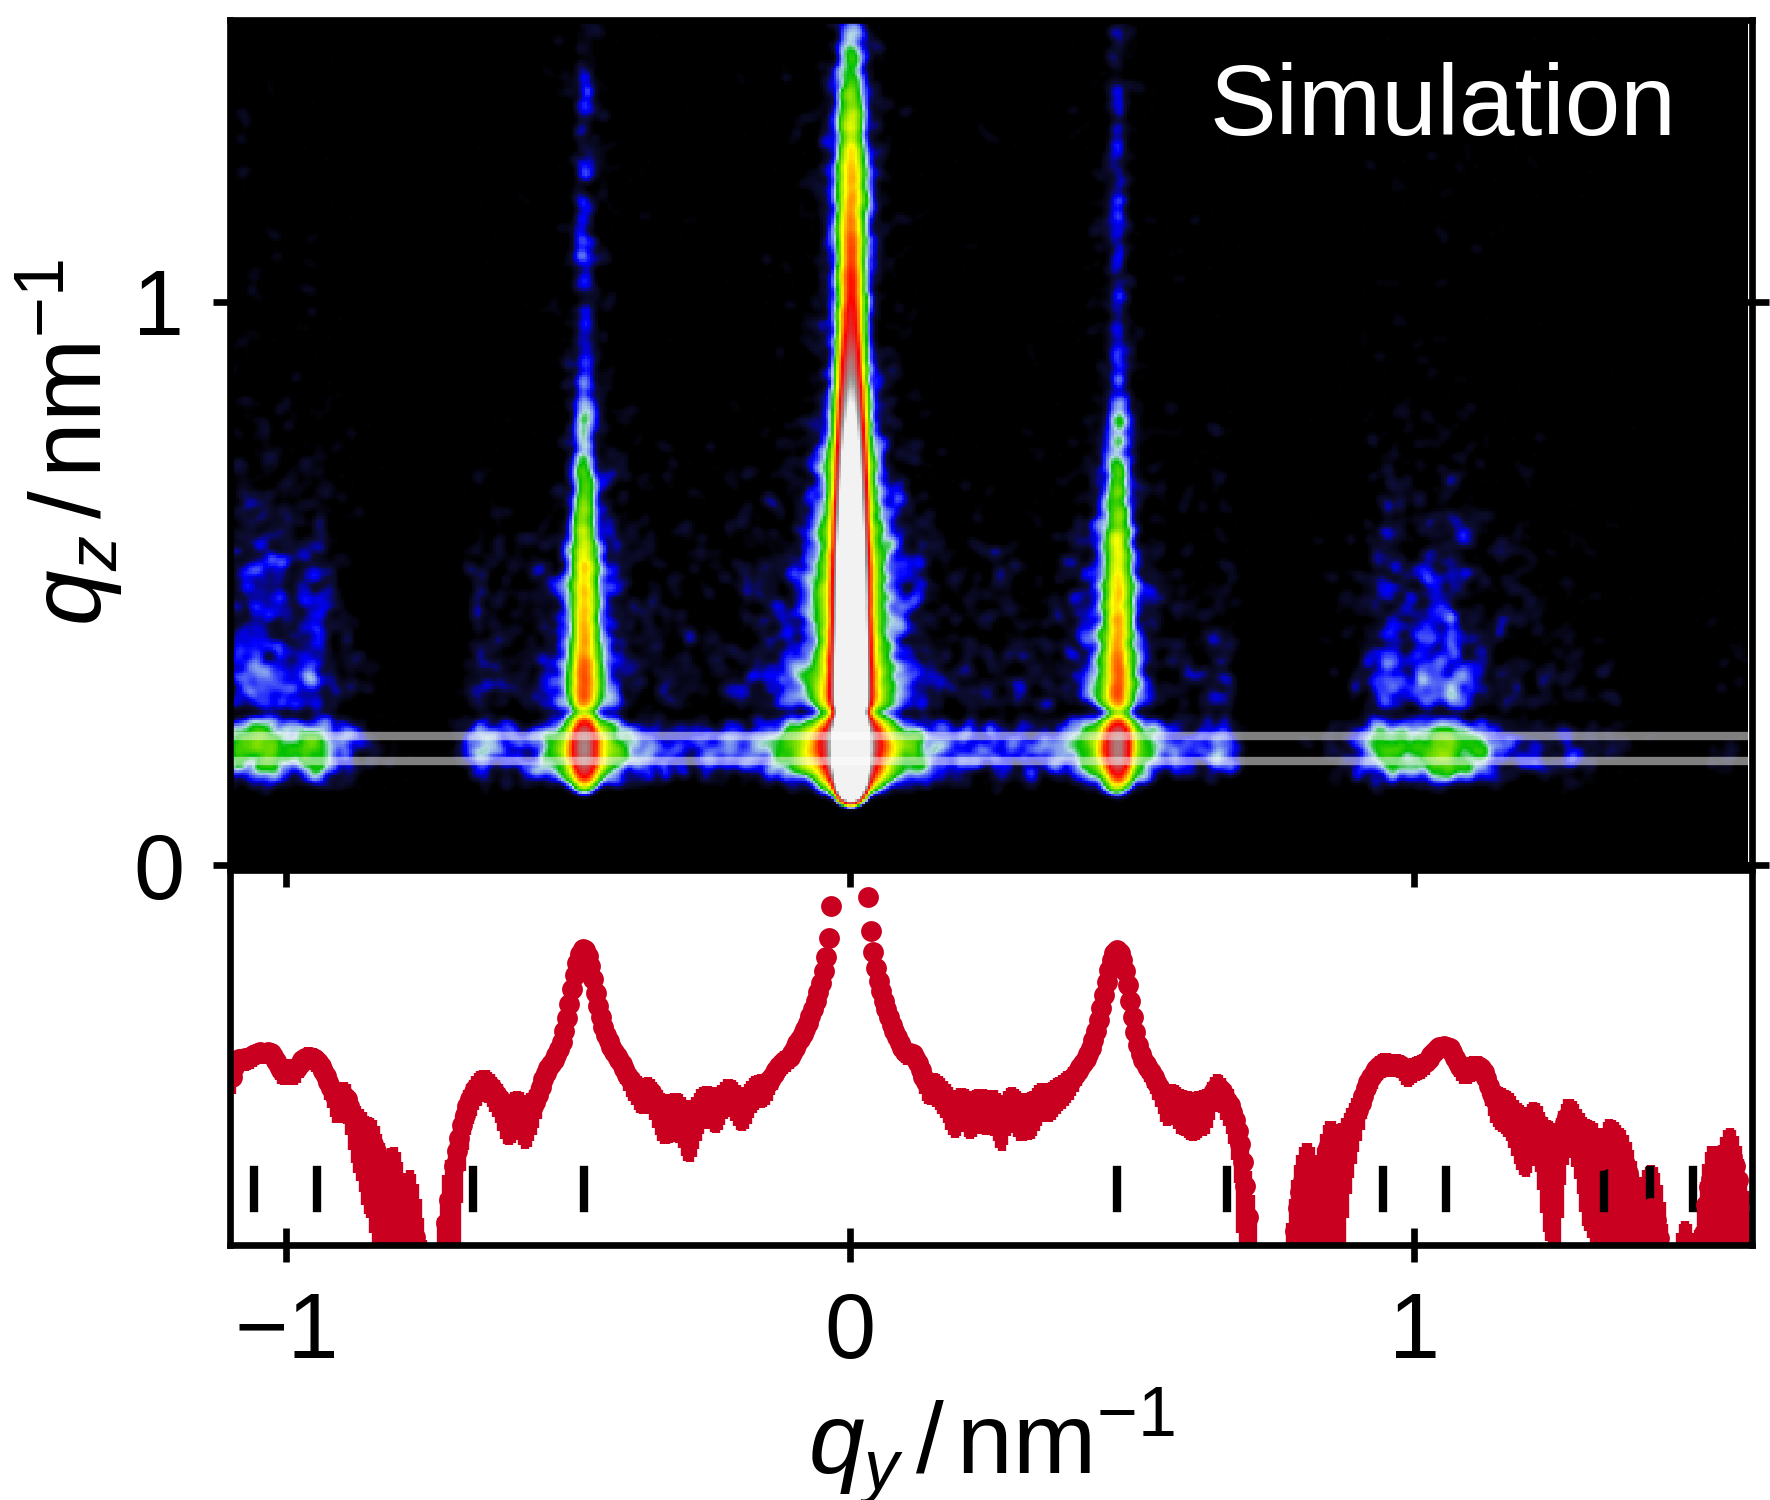
\includegraphics{monolayers_GISAXS_ParacrystalSimulation}
    \caption{\label{fig:monolayers:structure:ML-Ac-CoFe-C-2:GISAXS}GISAXS of ML-Ac-CoFe-C-2 measured at an incident angle of $\alpha_i \eq 0.15^\circ$ (left) and simulation of a paracrystal square lattice using the sample properties determined by complimentary experiments (right).}
  \end{figure}
  By grazing-incidence small-angle scattering, the in-plane order of ML-Ac-CoFe-C-2 is probed over a macroscopic area of the sample.
  In \reffig{fig:monolayers:structure:ML-Ac-CoFe-C-2:GISAXS} (left) the GISAXS of the sample is shown, with a projection of  the Yoneda band in the lower plot.
  The data show elongated peaks along $\mathit{q_z}$ and multiple sharp peaks emerging along $\mathit{q_y}$.
  The elongated peaks hint to a thin layer structure along the vertical direction, which has been confirmed by XRR in the previous section (\refsec{sec:monolayers:structure:verticalModel}), and the peak structure with respect to $\mathit{q_y}$ is related to the in-plane order.
  As the scanning electron microscopy images (\refsec{sec:monolayers:structure:semIntro}) suggest a square lattice order, in an initial step the first order peak is fitted to a Voigt function to determine the peak position and Lorentzian width corrected for the Gaussian peak broadening,  which result in $q_{10} \eq 0.4731(5) \unit{nm^{-1}}$ and $\gamma_{10} \eq 0.045(2) \unit{nm^{-1}}$.
  In the framework of a paracrystal (\refapp{ch:appendix:calculations:paracrystal}), this translates to a lattice constant of $13.28(2) \unit{nm}$, a coherence length of $L_{\mathrm{coh}} \eq 877(39) \unit{nm}$ and a nearest neighbour uncertainty of $1.63(4) \unit{nm}$.

  The values are used in the BornAgain software package \cite{Burle_2018_borna}, to simulate the two dimensional GISAXS data of nanocubes with a paracrystalline square lattice interference function shown in the right plot of \reffig{fig:monolayers:structure:ML-Ac-CoFe-C-2:GISAXS} and the parameters tabulated in \reftab{tab:monolayers:structure:squareArrayParacrystal:BornAgainSimulation}.
  The oleic acid layer includes hereby the lower and upper oleic acid layer of the XRR model discussed in \refsec{sec:monolayers:structure:verticalModel}, and is used to embed the square array of nanocubes.
  A three-dimensional visualization of the simulated structure is furthermore shown in \reffig{fig:monolayers:structure:paracrystal3d}.

  \begin{table}[!htbp]
    \centering
    \caption{\label{tab:monolayers:structure:squareArrayParacrystal:BornAgainSimulation}Parameters of the simulated nanocubes in a paracrystalline square lattice shown in \reffig{fig:monolayers:structure:ML-Ac-CoFe-C-2:GISAXS} determined from the pseudo-Voigt fit of the first order peak, the XRR characterization of the layer (\refsec{sec:monolayers:structure:verticalModel}) and the SAS characterization of the nanocubes (\refsec{sec:monolayers:nanoparticle:sas}).}
    \begin{tabular}{l | c}
      \hline
      \multicolumn{2}{c}{\textbf{Paracrystal}}\\
      \hline
      $a_{p-p} \, / \unit{nm}$                                        & $13.28$ \\
      $L_\mathrm{damp} \, / \unit{nm}$                                & $877$ \\
      $\sigma_\mathrm{pos.}\, / \unit{nm}$                            & $1.63$ \\
      \hline
      \multicolumn{2}{c}{\textbf{Layers}}\\
      \hline
      $d_{\ch{SiO2}}\, / \unit{nm}$                                   & $7.7$\\
      $d_{\mathrm{OA}}\, / \unit{nm}$                                 & $10.08$\\
      $\mathrm{SLD}_{\ch{Si}} \, / \unit{10^{-6} \angstrom^{-2}}$     & $20.06 - 0.35 i$\\
      $\mathrm{SLD}_{\ch{SiO2}} \, / \unit{10^{-6} \angstrom^{-2}}$   & $22.68 - 0.23 i$\\
      $\mathrm{SLD}_\mathrm{OA} \, / \unit{10^{-6} \angstrom^{-2}}$   & $8.52 - 0.01 i$ \\
      \hline
      \multicolumn{2}{c}{\textbf{Nanocubes}}\\
      \hline
      $a \, / \unit{nm}$                                              & $8.58$ \\
      $\sigma_a \, / \unit{\%}$                                       & $15.0$ \\
      $\mathrm{SLD}_\mathrm{Cube} \, / \unit{10^{-6} \angstrom^{-2}}$ & $41.21 - 3.00 i$ \\
      \hline
      \multicolumn{2}{c}{\textbf{Instrumental}}\\
      \hline
      $\alpha_i \, / \unit{^\circ}$                                   & $0.13$ \\
      $\lambda \, / \unit{\angstrom}$                                 & $1.3414$ \\
      $L_\mathrm{SDD} \, / \unit{mm}$                                 & $1733.5$ \\
      $\sigma_q \, /\unit{mm}$                                        & $0.254$ \\
      $I_\mathrm{beam} \, / \unit{10^9}$                              & $6.246$ \\
      $I_\mathrm{bg}$                                                 & $1$ \\
      \hline
    \end{tabular}
  \end{table}

  \begin{figure}[tb]
    \centering
    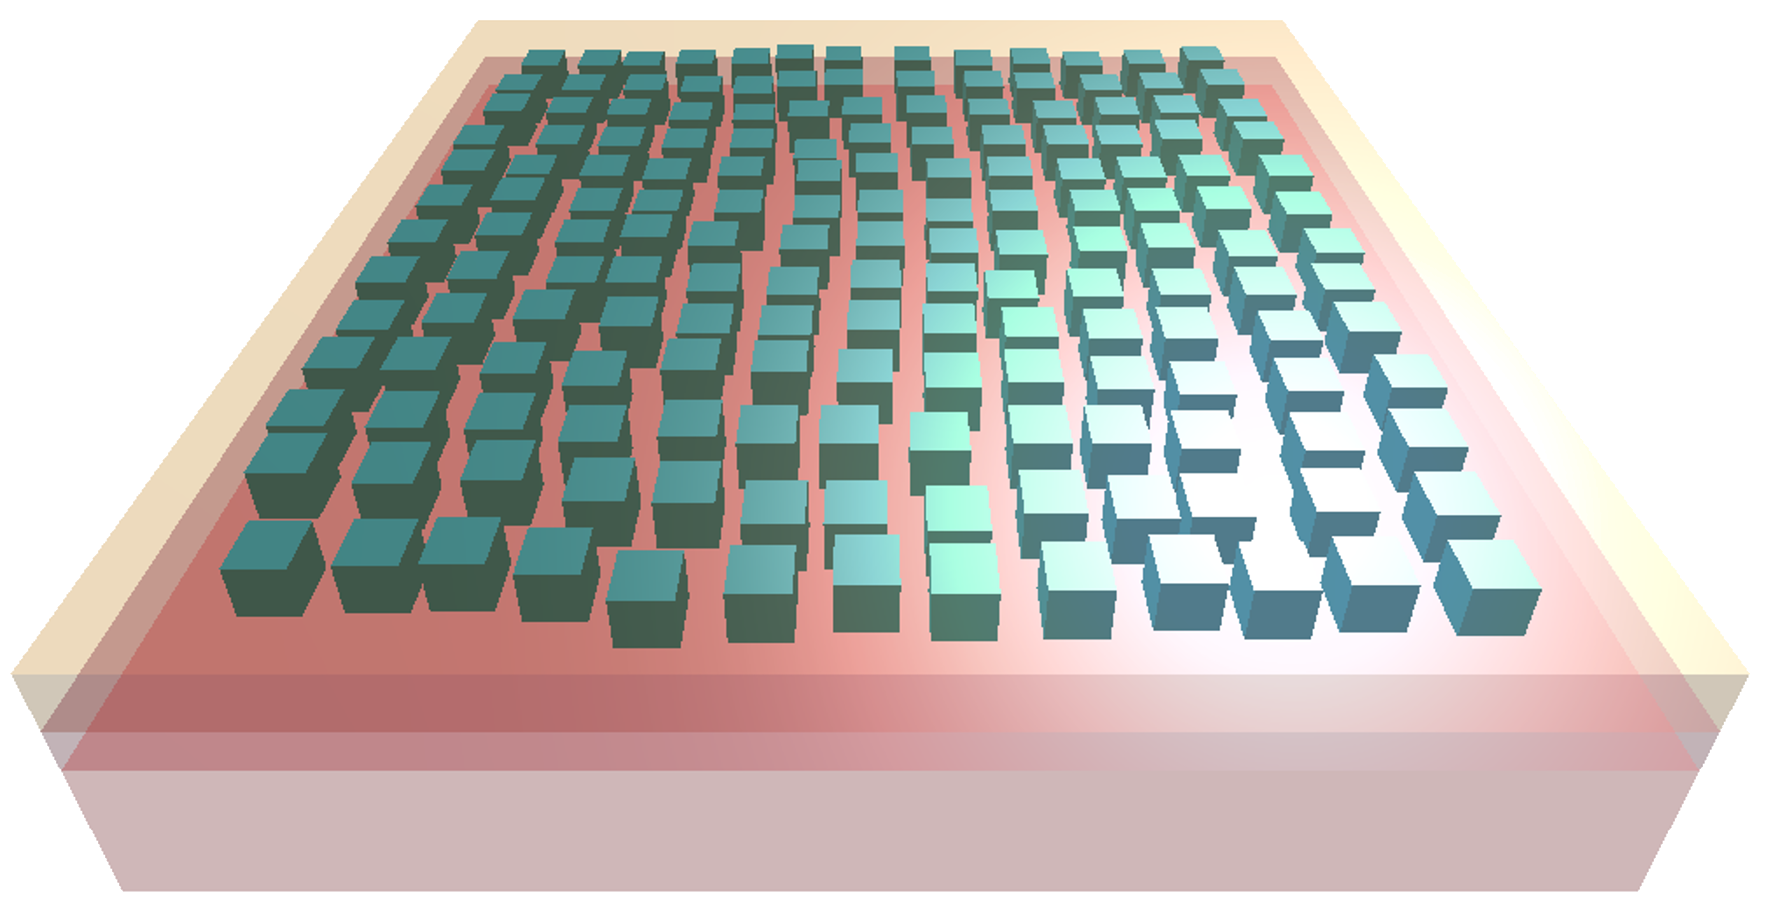
\includegraphics{monolayers_GISAXS_paracrystal3d}
    \caption{\label{fig:monolayers:structure:paracrystal3d}Three dimensional visualization of the simulated structure shown in the right plot of \reffig{fig:monolayers:structure:ML-Ac-CoFe-C-2:GISAXS}. The visualization was generated using the BornAgain software package \cite{Burle_2018_borna}.}
  \end{figure}

  The simulated GISAXS of the shown structure closely reproduces the experimentally obtained GISAXS data.
  The incident angle had to be readjusted to $\alpha_i \eq 0.13^\circ$ for the Yoneda line to be at the same height of the detector.
  Slight differences are observable in the intensity around $q_y \eq 0$, where the specular beam hits the detector and in the high $q_y$-range, where the experimental intensity drops quicker than simulated.
  Due to computational complexity, no roughness is included within the model and no distribution for the height position of the nanocubes.
  The approximation can be made responsible for the high $q_y$ behaviour, as typically roughness results in a quicker drop of the intensity.
\end{document}